% template
\section{Template matching}
we use templates with high SNR to cross-correlate with the continuous data to detect other events. The Figure \ref{fig:method} shows one example of this method.
\begin{figure}[htbp] 
\centering 
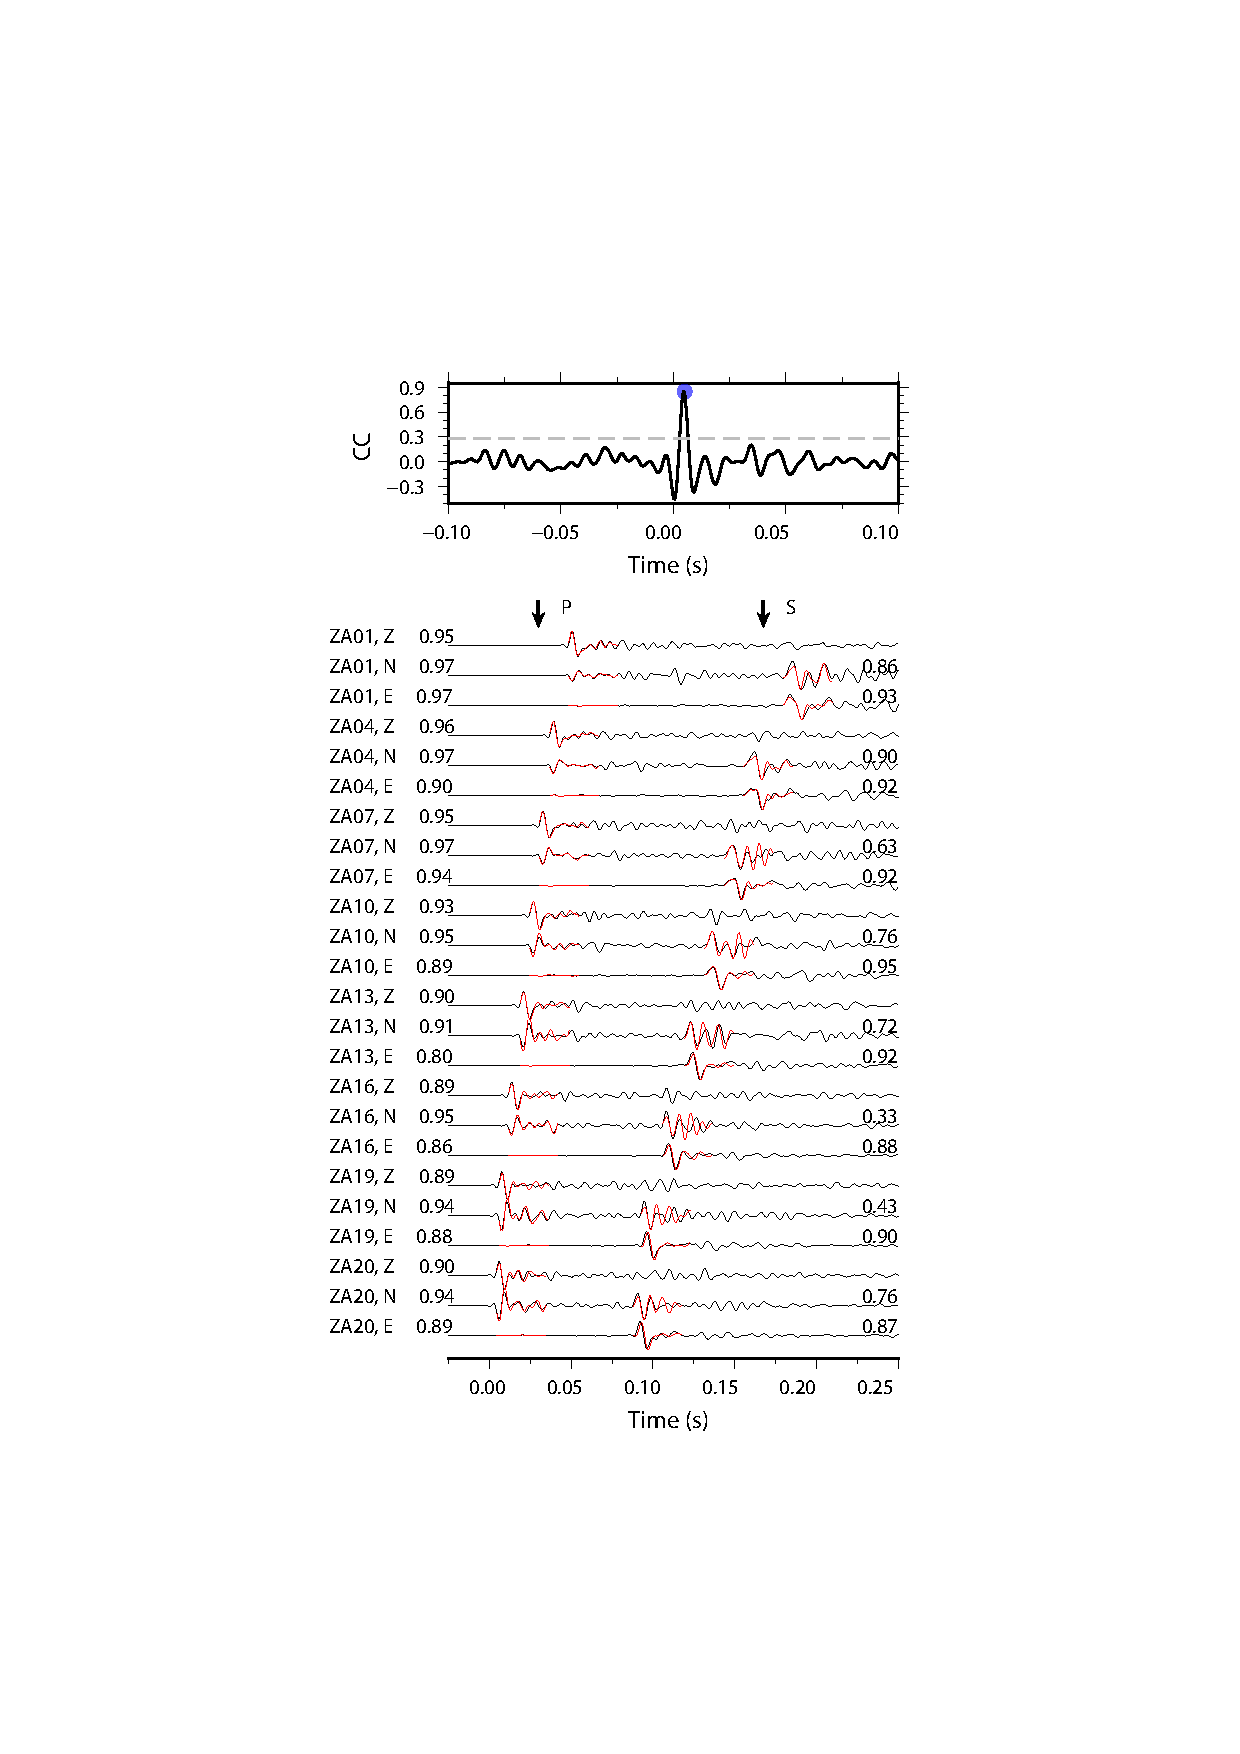
\includegraphics[height=6cm, width=3cm]{Template-search} 
\caption{\label{fig:method} (a) Stacked cross-correlograms. (b) Waveform comparison between the master event (red) and the target slave event (black) for the three components of several selected receiver levels.} 
\end{figure}
  In this project, we use 14 templates and detect 22 events. Among the 22 events, there are 8 events can obviously observed.

